\chapter{百年尺度的黄河流域人水关系演变}\label{cha:4}
第三章研究表明,人为压力和气候变化因素仅触发了黄河泥沙量的稳态转换,黄河流域在千年尺度上是由层级制度主导的“洪泛-响应”关系。除此之外,非中央政府主导的开发利用、生产贸易、综合治理等因素,尚没有显著影响人水关系稳态。而现代黄河流域人水关系出现的关键变化之一就是对黄河流域全面的综合开发、利用、以及治理。黄河流域的战略瓶颈已经由保护黄河泛滥转向应对高质量发展面临的水资源短缺、人水关系不协调问题之上。第三章研究已经表明,这是19世纪以降短短百余年间经济社会高速发展带来的问题,而新中国成立以来,高强度的黄河流域综合治理,使得近六十年间黄河流域人水关系的演变模式与过去千年相比显得截然不同。

首先在流域内部,积累的取水压力让这个位于干旱-半干旱区的流域迅速不堪重负,取水量一度接近年径流的$80\%$,其中近$90\%$均为农业取水。因此,黄河自1970年代开始频繁断流,这引起中央高度重视,开始采取一系列水资源管理的工程、非工程措施来协调水资源供需矛盾。与此同时,大规模的经济建设和城市发展也让宝贵水资源的流域内分配成为了挑战。而跨区域贸易带来了水资源以农产品形式向流域外的转移,让水资源分配的问题变得更加复杂严峻。因此,黄河流域已从过去的调水调沙与防洪等河道内外的“工程问题”,转向了“谁、在何时得到水”的流域层面的“非工程问题”,这是近现代人水关系演变的体现。而这种稳态转变何时发生、如何发生,仍需要定量研究。本章在黄河流域市级统计数据的支持下,利用断点识别、复杂网络分析等方法量化分析了上世纪七十年代以来的黄河人水关系演变过程及驱动因素。

黄河流域是世界上第五大、最富沉积物的河流,由于地质和人类历史的原因,需要综合的水治理
\cite{mostern2021,best2019}。
自20世纪60年代以来,水库、堤坝和保护措施等治理措施已经遏制了数千年来高沉积物负荷所困扰的问题
\cite{wang2016e,song2020a}。
然而,最近出现了新的挑战,如流量减少和水资源枯竭,导致了用水调节和跨流域的水转移——不同的重点水治理策略
\cite{wang2019c}。
目前,还不可能完全解决长江流域水资源压力、生态系统服务之间的权衡、不同区域的不平衡发展问题,使各方都满意
\cite{wohlfart2016a}。
由环境、经济、社会和政治因素引发的治理挑战导致长江流域成为世界上治理最密集的大型流域之一。
因此,确定长江流域内水治理的政权变化,可以为快速变化的大流域以及治理如何应对其可持续性挑战提供重要的见解。

\section{研究方法与数据来源}\label{ch4:methods}

\subsection{分析框架}

% 根据本研究的定义,人类活动主导下的人\textendash{}水关系是社会\textendash{}水文二元循环中由人类主导的决策模式
% 而水治理(Water Governance)是指影响水使用和管理的政治、社会、经济、和行政系统相互作用的全部过程,本质上是关于``谁获得水,何时获得水,如何获得水''(``who gets water, when and how'')。
联合国开发计划署(UNDP)提出\cite{mariajacobson2013},水治理决定了与水有关的三个核心方面:``什么时候有多少水用?''、``水如何为人类福祉提供不同的生态系统服务?''以及``谁能平等有效地用水?''——简而言之,水治理是决定水资源``稀缺情况''、``使用目的''、和``分配方式''的关键。
为此,本章研究将水治理的三个核心方面(``稀缺情况''、``使用目的''和``分配方式'')各自选择指标进行量化,对它们进行等权平均得到综合水治理指数(Integrated Water Governance Index, IWGI)用以识别水治理的稳态变化(图\ref{ch4:fig:framework})。
然后,通过将该指数应用在黄河这个典型的人类活动主导的流域,利用突变点检测的方法分析了$1965\sim2013$年间IWGI的变化,展示该IWGI如何有助于检测和描述复杂的水治理稳态变迁。
最后,在综合分析了水资源供需、经济发展、环境变迁,以及制度变化后,本章解释了黄河流域水治理稳态变化的主要驱动因素,并总结提出了一个过渡模式,为人类活动主导大河流域面临的治理挑战提供了抓手。

\begin{figure}[!ht]
\centering
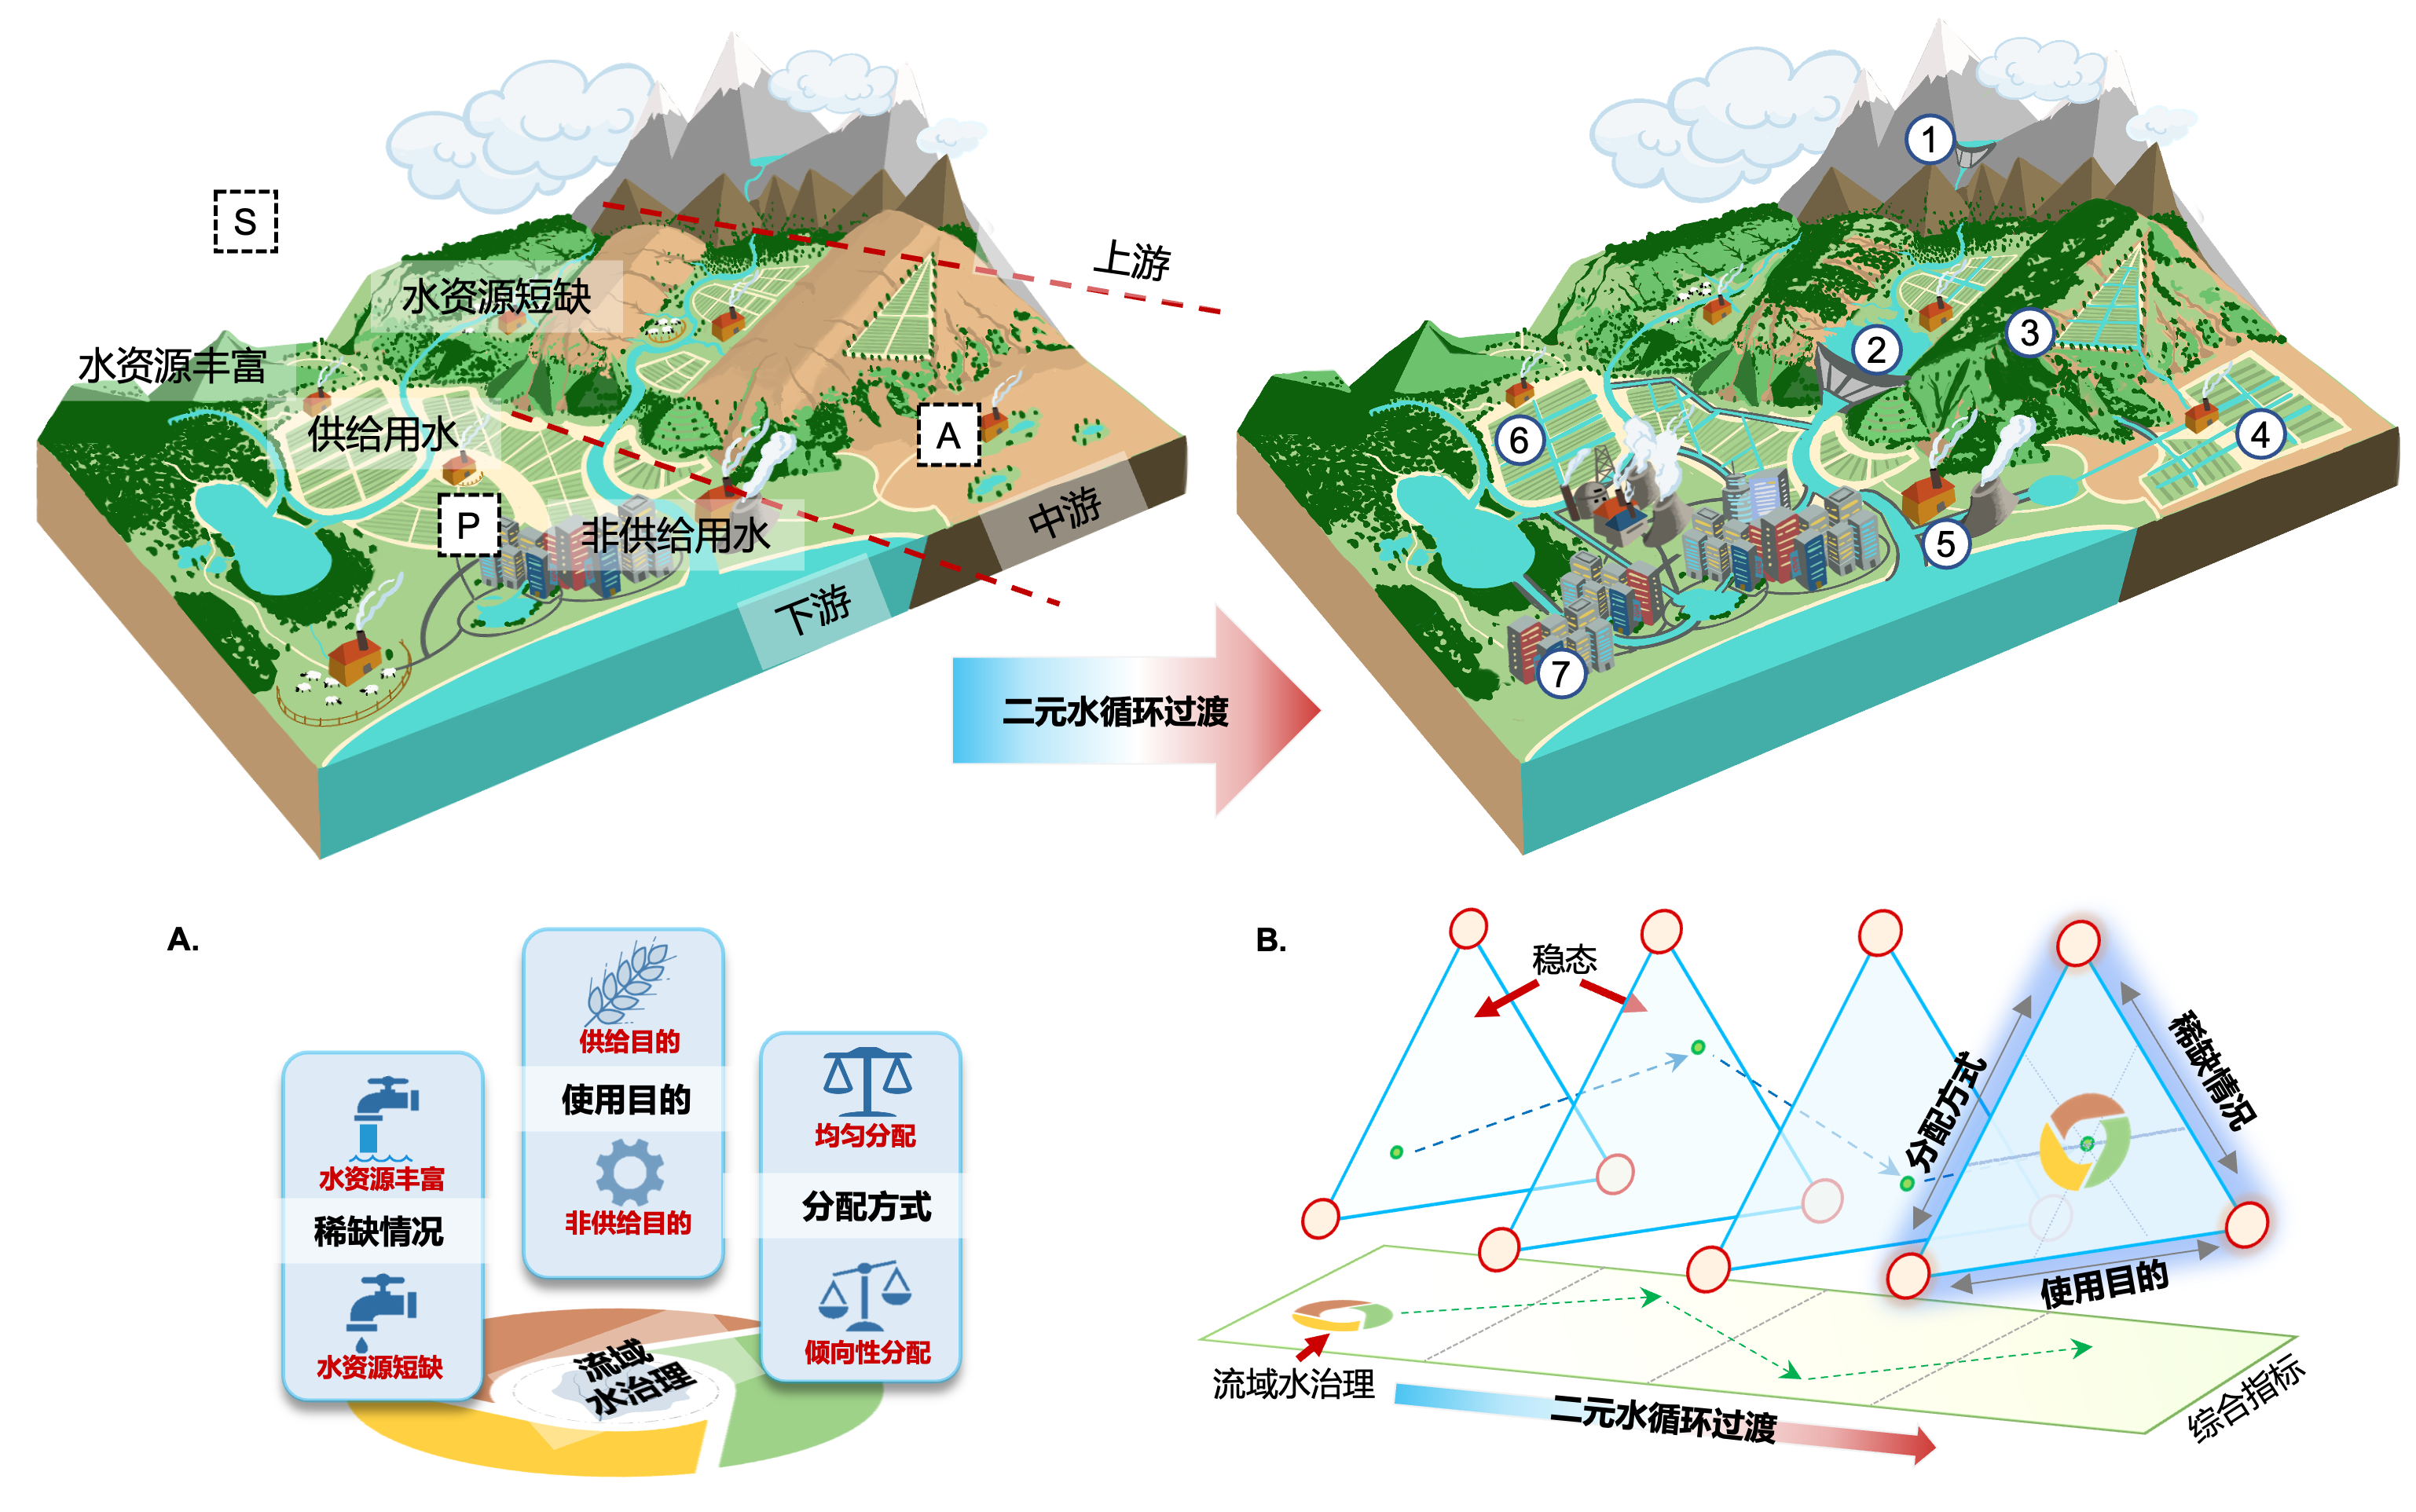
\includegraphics[width=\textwidth]{img/ch4/ch4_framework.png}
\caption[定量识别流域水治理转变的分析框架]{
    定量识别流域水治理转变的分析框架。
    \textbf{A} 利用综合水治理指数(IWGI)识别水自然\textendash{}社会二元循环过渡时期中的水治理机制,可以从稀缺情况(S)、使用目的(P)和分配方式(A)这三方面切入,三者会随着人类活动主导社会\textendash{}水文循环而变化。
    例如,水库建设(\ding{172}和\ding{173})可以缓解局地水资源压力;集约化灌溉农业的发展(\ding{174})以及能源和工业增长(\ding{175})会改变水的利用方式;输水系统控制了流域系统的水分配(\ding{176}和\ding{177})。
    \textbf{B} IWGI方法结合三个方面的相应指标,因此其突变可以指示水治理的稳态转换。}\label{ch4:fig:framework}
\end{figure}

\subsection{研究区域划分}\label{ch4:sec:region}

为便于研究的计算需要,本章参考前人研究和黄河水利委员会的标准将黄河流域划分为四个区域\cite{shuilibuhuangheshuiliweiyuanhui2010,wang2019c},以四个重要的控制水文站反映各区域的径流变化,各区域特点鲜明,便于后文对水资源治理的变化原因进行分析:

黄河源区(SR,控制水文站为唐乃亥站)人口稀少,经济欠发达,主要生态功能是水源涵养,黄河超$50\%$的天然径流来自这里。
黄河上游(UR,控制水文站为头道拐站)人均灌溉土地面积最高的区域,大量引黄河水发展灌溉农业,但灌溉效率相对较低。
黄河在中游(MR,控制水文站为花园口站)流经著名的富沙区——黄土高原,作为土壤侵蚀风险最高的地区,是黄河产沙最多的地区,近三十年的``退耕还林''生态工程显著改变了这里的土地利用覆被。
黄河下游(LR,控制水文站为利津站)人口密集,传统的农业发达地区,也曾是最大的黄河水资源使用地区。随着产业升级和节水工程的持续实施,农业用水的比重不断下降,但仍是总用水最多的地区。


% % 补充图片1:研究区示意图
% \begin{figure}[hbtp!]
% \centering
% 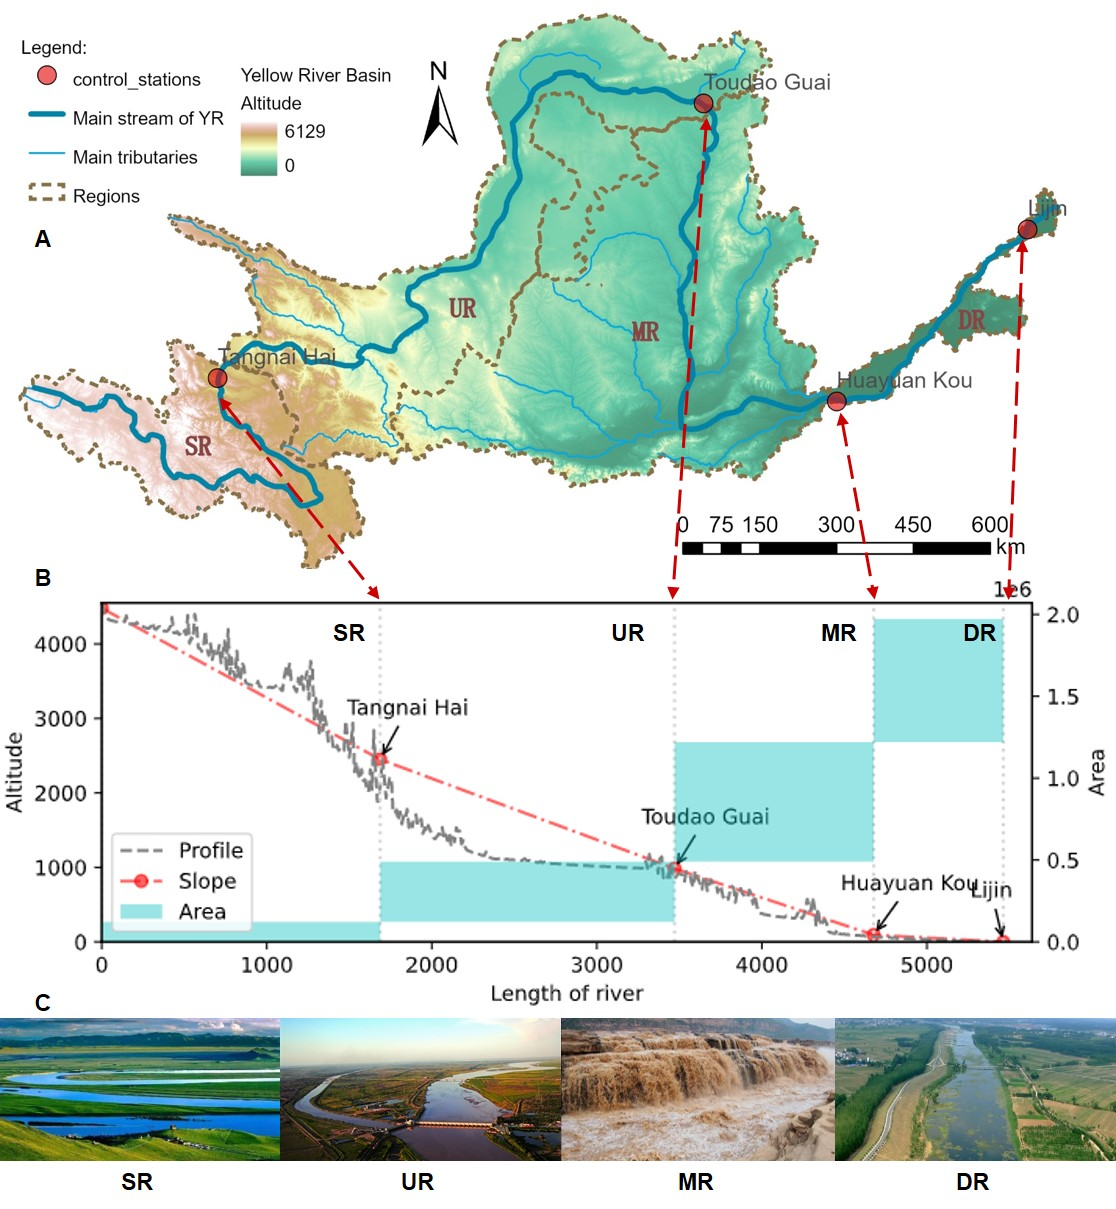
\includegraphics[width=\textwidth]{img/ch4/s1_study_area.jpg}
% \caption[黄河流域子区域划分]{黄河流域子区域划分。
%     \textbf{A.}黄河流域划分示意图(SR:源区,UR:上游,MR:中游,DR:下游);
%     \textbf{B.}黄河主河道剖面图,四个水文观测站分别控制SR、UR、MR和DR;
%     \textbf{C.}黄河流域不同地区的典型景观。}\label{fig:YRB}
% \end{figure}

\subsection{综合治理指数}

\subsubsection{综合指标构建方法}

% 将三者合一起,即:
如本章前文介绍以及框架图~\ref{ch4:fig:framework}所示,本研究定义的水资源治理综合指数(IWGI)应结合水治理的三个方面(``稀缺情况(S)''、``使用目的(P)''和``分配方式(A)'')。
由于每个指标维度都有升高和降低两个方向,在整合指标前应假设随着人类活动主导社会\textendash{}水文循环的进程,三者在其中某个方向对齐:
\begin{equation}
    Transformation \propto S*P*A
\end{equation}

接下来为三个方面选择了一个指标($I_x$, $x=S$, $P$,或$A$,分别对应``稀缺情况(S)''、``使用目的(P)''和``分配方式(A)'',来有效地量化这些方面,并将上式转化为自然对数,便于计算各指标对综合指数变化的贡献:
\begin{equation}
    Transformation \propto \ln(I_S) + \ln(I_P) + \ln(I_A)
\end{equation}
那么,综合水治理指数(IWGI)是标准化指标$I'_x$的平均值:
\begin{equation}
    IWGI = (I'_S + I'_P + I'_A) / 3
    \label{ch4:eq:IWGI}
\end{equation}
其中:
\begin{equation}
    I'_x = (I_x - I_{x, \min}) / (I_{x, \max} - I_{x, \min})
\end{equation}

对三个方面各自的指标选取如下文所述。

\subsubsection{子指标:水的稀缺情况}

水的``稀缺情况''既取决于气候能提供稀缺情况资源,还取决于灌溉和工业等经济活动的需求,更可以被水库蓄水、跨流域调水等工程所人为改变\cite{qin2019,wada2014,huang2021}。
本章研究采用Qin等人(2019)提出的稀缺性\textendash{}弹性\textendash{}易变性(SFV)水稀缺指数来评价``稀缺情况''的问题\cite{qin2019}。
这一指标考虑了管理措施(如水库的建设)和用水结构变化(有些用水方式如能源用水是难以被短期替代的),对水资源短缺情况做出评估。
此外,SFV指数从发展的角度关注水资源的动态,同时考虑了水资源的灵活性和易变性(例如气候差异带来的降水波动),是衡量水资源压力\cite{qin2019}时间变化的有效指标。
整个黄河流域的水分胁迫指标$I_S$为本章划分的四个二级区域$i$——源区(SR)、上区(UR)、中游(MR)、和下游(DR)指数$SFV_{i}$的平均值:

\begin{equation}
    I_S = \frac{1}{4} * \sum_{i=1}^4 SFV_{i}
    \label{ch4:eq:scarcity}
\end{equation}

其中$SFV_i$为区域$i$的SFV指数$SFV_i$,SFV结合了以下三个指标:

首先,对于稀缺性(Scarcity, S),$A_{i, j}$为区域$i$在第$j$年的耗水量占多年平均径流量的比例(本研究将为黄河流域划分为四个子区域,见\ref{ch4:sec:region}\nameref{ch4:sec:region}):

\begin{equation}
    A_{i, j} = \frac{WU_{i,j}}{R_{i, avg}}
\end{equation}

% TODO 完整的不灵活用水分类?
其次,对于灵活性(Flexibility, F),$F_{i, j}$是第$i$年和第$j$区域的不灵活用水$WU_{inflexible}$(例如能源行业冷却用水或人类和牲畜)占平均多年径流量的比例:

\begin{equation}
    F_{i, j} = \frac{WU_{i, j, inflexible}}{R_{i, avg}}
\end{equation}

最后,易变性(Variability, V)还考虑了水库容量和蓄水对自然径流波动的积极影响:
\begin{gather}
    C_i = C1_i * (1 - C2_i) \\
    C1_{i, j} = \frac{R_{i, std}}{R_{i, avg}} \\
    C2_{i} = \frac{RC_{i}}{R_{i, avg}}, \ if RC < R_{i, avg} \\
    C2_{i} = 1, \ if RC \geq  R_{i, avg}
\end{gather}

上式中,$R_{i, avg}$为$i$区域的平均径流量,$RC_i$为$i$区域水库的总库容,$R_{i, std}$为$i$区域径流量的标准差。

最后,该方法将三个指标(稀缺性S、灵活性F和易变性V)以相同的权重进行归一化后加权计算出$SFV$指标:

\begin{gather}
    V = \frac{A_{normalize} + B_{normalize} + C_{normalize}}{3}\\
    a = \frac{1}{V_{\max} - V_{\min}};\\
    b = \frac{1}{V_{\min} - V_{\max}} * V_{\min}\\
    SFV = a * V + b
\end{gather}


\subsubsection{子指标:水的使用目的}

水的``使用目的''与水能够提供的生态系统服务有关,但目前对文化、调节服务等缺乏成熟统一的评估框架,且受限于数据,本研究仅将用水分为供给用途(例如,日常饮用和食品生产)和非供给用途(例如能源冷却用水)的用水\cite{liu2017,florke2018,jaeger2019}。
本章研究使用供给服务目的在全部用水量中所占比例(Provisioning Purpose Shares, PPS)作为量化``使用目的(P)''$I_P$的指标。

\begin{equation}
    PPS = \frac{WU_{pro}}{WU_{pro} + WU_{non-pro}}
\label{ch4:eq:priority}
\end{equation}

其中($WU_{pro}$)为供给服务用水,包括家庭用水、灌溉用水和牲畜用水;非供给服务的用水($WU_{non-pro}$)包括工业用水和城市服务用水。
% 本章研究将牲畜用水、城乡生活用水和农业用水作为供应用水,因为它们直接服务于生存。其他的是非供应:服务和工业用水,因为它们主要为经济服务。

\subsubsection{子指标:水的分配方式}

最后,水的``分配方式''并非取决于区域的社会经济水平和自然环境背景,流域的水资源分配还会受到流域系统调度的工程(如水库统一调度)、非工程因素(如水资源分配制度)的影响\cite{schmandt2021,speed2013}。
本章借鉴使用熵作为刻画分配均匀程度的指标(式\ref{ch4:eq:allocation})\cite{peet1974},当不同区域间水资源使用完全平均时,当完全平均分配时该指标达到最大值$I_{A, \max} = 1$,当区域的用水量相差悬殊时$I_A \in [0, 1]$趋近于零。

\begin{equation}
    I_A = \sum_{i=1}^N - \log(p_{i}) * p_{i}
    \label{ch4:eq:allocation}
\end{equation}

其中$p_{i}$为区域$i$与整个流域的水量比例,由于本研究将黄河流域分为源区和上中下游,因此$N=4$。

\subsection{突变点检测}

本章研究采用Pettitt提出的的突变点检测方法,在不假设数据分布的情况下,对时间序列数据的单个变化点进行检测\cite{pettitt1979},它测试的原假设$H_0$是:变量不存在变化趋势差异,备择假设则为存在一个显著的趋势变化点。
通过将随机变量序列分为$\mathrm{x}_{1}, \mathrm{x}_{1}, \ldots, x_{t_{0}}$和$x_{t_{0}+1}, x_{t_{0}+2}, \ldots, x_{T}$表示的两段,如果每段都有一个共同的分布函数,即$F_1(x)$、$F_2(x)$和$F_1(x) \neq F_2(x)$,则在$t_0$处确定变化点。

为实现变化点的识别,定义统计指标$U_{t,T}$如下:

\begin{equation}
    U_{t, T} = \sum_{i=1}^t\sum_{j=t+1}^T sgn(X_i - X_j), 1 \leq t < T
\end{equation}

其中:
\begin{equation}
    \operatorname{sgn}(\theta)= \begin{cases}1 & \text { if } \theta>0 \\ 0 & \text { if } \theta=0 \\ -1 & \text { if } \theta<0\end{cases}
\end{equation}

找到最可能的变化点$\tau$,其值满足$K_{\tau} = \max|U_{t, T}|$,与值$K_{\tau}$相关的显著性概率近似计算为:

\begin{equation}
    p=2 \exp \left(\frac{-6 K_{\tau}^{2}}{T^{2}+T^{3}}\right)
\end{equation}

给定某个显著性水平$\alpha$,如果$p < \alpha$,则拒绝原假设并得出结论$x_{\tau}$是水平$\alpha$的显著突变点。

本章研究使用$\alpha = 0.001$作为显著性$p$的阈值,这意味着统计上显著的变化点判断有效的概率大于$99.9\%$。
迭代使用Pettitt算法:反复识别一个突变点从而将时间序列分为该时间点前后两段,并再次分别对两序列进行分析,直到检测到所有显著的突变点。
虽然接下来的结果展示的是阈值$\alpha = 0.001$的结果(识别出两个断点),但是经过敏感性分析,从$0.0005$到$0.05$的阈值范围选取都不影响本研究结果的鲁棒性(参见图\ref{ch4:fig:sensitivity})。

\begin{figure}[!ht] % use float package if you want it here
    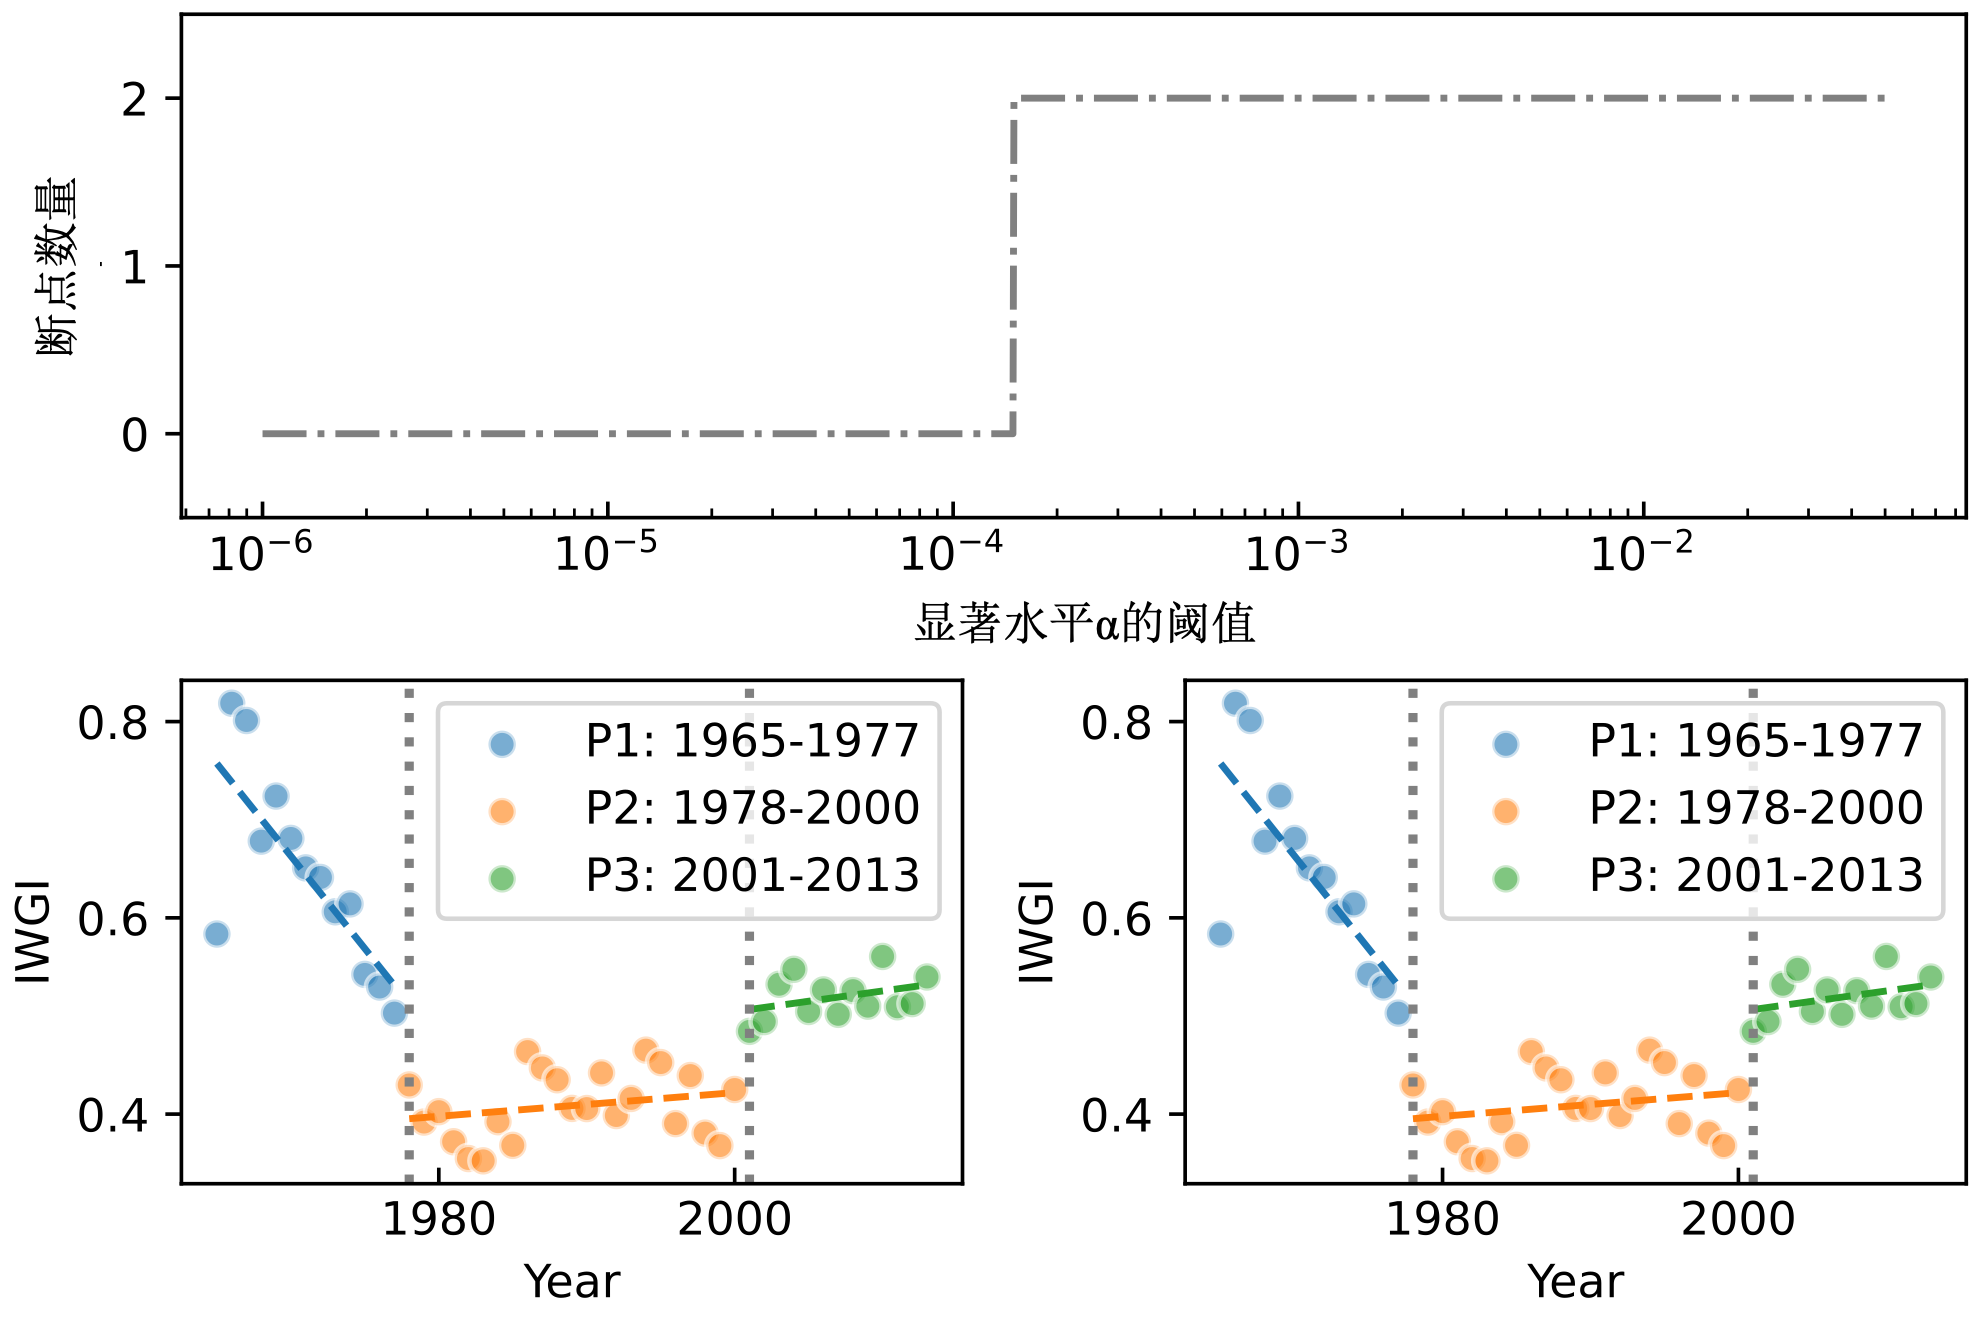
\includegraphics[width=\textwidth]{img/ch4/ch4_sensitivity.png}
    \caption[突变点检测中显著性阈值选取的敏感性测试]{突变点检测中显著性阈值选取的敏感性测试结果。
    \textbf{A} 选取不同阈值$\alpha$后识别的突变点个数,所有的方案都识别了两个断点。
    \textbf{B} 阈值选取为 $\alpha=0.0005$.
    \textbf{C} 阈值选取为 $\alpha=0.05$.}\label{ch4:fig:sensitivity}
\end{figure}

\subsection{数据来源}

% % Table generated by Excel2LaTeX from sheet '数据集'
\begin{table}[htbp]
    \centering
    \caption{数据分类与来源}
      \begin{tabularx}{\textwidth}{LLLLL}
      \toprule
      数据集   & 数据类型  & 空间尺度  & 时间尺度  & 数据来源 \\
      \midrule
      行政区水资源利用 & 统计    & 市级行政单元 & $1965-2013$ & Zhou等人2020 \\
      子流域水资源使用 & 统计    & 二级子流域 & $2003-2019$ & 水资源公报 \\
      GDP数据 & 统计    & 省级行政单元 & $1949-2019$ & 万德数据库 \\
      水库数据集 & 水文    & 站点数据  & $1949-2015$ & Wang等人2019 \\
      实测泾流量 & 水文    & 站点数据  & $1949-2019$ & Wang等人2019 \\
      黄河流域相关法律 & 文献    & 流域相关文件 & $1949-2013$ & 黄河流域规划 \\
      黄河水利委员会历史 & 文献    & 流域相关文件 & $1949-2002$ & 黄河水利委员会档案馆 \\
      黄河大事件 & 文献    & 流域相关文件 & $1949-2015$ & 黄河水利委员会档案馆 \\
      \bottomrule
      \end{tabularx}%
    \label{ch4:tab:data_source}%
\end{table}%
  

为了计算IWGI,使用了三个数据集:水库、实测径流、和用水。
水库数据集由Wang等人~\cite{wang2019c}收集,其中包括1956年以来新建的重要水库。
在所有水库中,黄河水利委员会已经将主要用于调节和管理的水库称为``主要水库''(见\url{http://www.yrcc.gov.cn/hhyl/sngc/})。
此外,每年的实测径流数据来自《黄河泥沙公报》(\url{http://www.yrcc.gov.cn/nishagonggao/}),分别由四个控制站(唐乃亥、头道拐、花园口、利津)在黄河的不同河段(源区、上游、中游、下游)进行测量得到。
水资源利用数据来源于Zhou等人\cite{zhou2020}发布的中国国家长期水资源利用数据集(NLWUD),包括地级市不同部门的用水量、用水经济变量和用水强度,我们以$95\%$相交面积为阈值筛选该数据集中的地级市,得到属于黄河流域的子数据集。

为了分析其变化的原因,灌溉面积、工业增加值和服务业总增加值以及用水强度数据也来自NLWUD数据集~\cite{zhou2020}。
此外,还使用了两个水治理政策数据集:法律政策和``大事件''文件数据集。
法律政策记录(表~\ref{ch4:tab:policies})来源于2013年公开批准的``黄河流域综合规划'',其中回顾了建国以来全流域尺度上的重要法律法规。
与黄河有关的``大事件''的原始文件则来自黄河水利委员会的记录和汇编(\url{http://www.yrcc.gov.cn/hhyl/hhjs/})。

本研究中使用或分析的所有数据,包括水库数据集、测量径流、用水数据集、规律和大事件,都已储存在公开获取的数据仓库中(\url{https://doi.org/10.5281/zenodo.7955500}~\cite{shuang_song_2023_7955500})。

% Table generated by Excel2LaTeX from sheet '黄河流域法律政策'
\begin{table}[htbp]
    \centering
    \caption{黄河流域法律政策}
      \begin{tabularx}{\textwidth}{L p{1.5cm} L}
      \toprule
      法律或政策名称 & \multicolumn{1}{l}{施行或修订时间} & 颁布机构 \\
      \midrule
      中华人民共和国水法 & 1,988 & 全国人民代表大会常务委员会 \\
      中华人民共和国水法  修正 & 2,002 & 全国人民代表大会常务委员会 \\
      中华人民共和国水法  第一次修订 & 2,009 & 全国人民代表大会常务委员会 \\
      中华人民共和国水法  第二次修订 & 2,016 & 全国人民代表大会常务委员会 \\
      中华人民共和国水污染防治法 & 1,984 & 全国人民代表大会常务委员会 \\
      中华人民共和国水污染防治法  修正 & 1,996 & 全国人民代表大会常务委员会 \\
      中华人民共和国水污染防治法  第一次修订 & 2,008 & 全国人民代表大会常务委员会 \\
      中华人民共和国水污染防治法  第二次修订 & 2,018 & 全国人民代表大会常务委员会 \\
      取水许可和水资源费征收管理条例 & 2,006 & 中华人民共和国国务院 \\
      取水许可和水资源费征收管理条例  第一次修订 & 2,017 & 中华人民共和国国务院 \\
      黄河水量调度条例 & 2,006 & 中华人民共和国国务院 \\
      黄河可供水量分配方案 & 1,987 & 中华人民共和国国务院 \\
      取水许可管理办法 & 2,008 & 中华人民共和国水利部 \\
      取水许可管理办法  第一次修订 & 2,015 & 中华人民共和国水利部 \\
      取水许可管理办法  第二次修订 & 2,017 & 中华人民共和国水利部 \\
      黄河水量调度条例 & 2,006 & 中华人民共和国国务院 \\
      黄河可供水量年度分配及干流水量调度方案 & 1,998 & 国家发展计划委员会,水利部 \\
      黄河水量调度管理办法 & 1,998 & 国家发展计划委员会,水利部 \\
      黄河水权转换管理实施办法 & 2,004 & 水利部 \\
      取水许可和水资源费征收管理条例 & 2,006 & 中华人民共和国国务院 \\
      取水许可证制度实施办法 & 1,993 & 中华人民共和国国务院 \\
      建设项目水资源论证管理办法 & 2,002 & 国家发展计划委员会,水利部 \\
      水利工程管理体制改革实施意见 & 2,006 & 中华人民共和国国务院 \\
      \bottomrule
      \end{tabularx}%
    \label{ch4:tab:policies}%
  \end{table}%
  

\subsection{数据分析}

\subsubsection{相关分析与显著性检验}

皮尔逊相关系数(Pearson correlation coefficient,通常用 $r$ 表示)是用于衡量两个连续变量之间线性关系强度的指标。它的值范围在 $-1$ 到 $1$ 之间,其中 $-1$ 表示完全负相关,$1$ 表示完全正相关,$0$ 表示无相关性,本研究使用该指标反映某时段内IWGI的趋势同哪些子指标变化趋势更密切,为了计算两个变量之间的皮尔逊相关系数,我们可以使用以下公式\cite{freedman2007}:

\begin{equation}
    r = \frac{\sum_{i=1}^{n}(x_i - \bar{x})(y_i - \bar{y})}{\sqrt{\sum_{i=1}^{n}{(x_i - \bar{x})}^2}\sqrt{\sum_{i=1}^{n}{(y_i - \bar{y})}^2}}
\end{equation}

其中,$x_i$ 和 $y_i$ 分别表示第 $i$ 个观察值,$\bar{x}$ 和 $\bar{y}$ 分别表示 $x$ 和 $y$ 的均值,$n$ 表示观察值的数量。计算出皮尔逊相关系数后,我们需要进行显著性检验来确定这种关系是否具有统计显著性。这里我们使用 $t$ 检验来计算显著性水平。根据 $r$ 和样本大小,我们可以计算 $t$ 值\cite{freedman2007}:

\begin{equation}
    t = \frac{r\sqrt{n-2}}{\sqrt{1-r^2}}
\end{equation}

根据统计量$t$的值查表判断显著性水平,如果 $p$ 值低于预先设定的显著性水平$0.01$,则我们可以认为两个变量之间的关系具有统计显著性。在实际应用中,我们使用 scipy 1.10.1~\cite{2020SciPy-NMeth}完成这些计算。

\subsubsection{基于平均的指标贡献度}

本研究中,表征稀缺情况的SFV指数就是稀缺性(S)、弹性(F)、易变性(V)三个指标在不同区域(源区、上游、中游、下游)之间的等权重平均(见式\ref{ch4:eq:scarcity}),综合水治理指标(IWGI)则是稀缺情况、使用目的、分配方式三个子指标取对数后的等权重平均(见式\ref{ch4:eq:IWGI})。
对此类指数,本研究中使用如下方法计算某时段某子指标($X$)对总指标变化(或指标/地区均值)的贡献度$Contribution_{X}$:

\begin{equation}
    Contribution_{X} = \Delta_{X} / \Delta_{Index}
\end{equation}

其中$\Delta_{X}$是该子指标在给定时段(从$t=start$到$t=end$)内的总变化值,$\Delta_{I}$是该子指标参与贡献的总指标总变化,两者都可以使用如下公式计算:

\begin{equation}
    \Delta=\sum_{t=start}^{end}(X_{t}-X_{t-1})
\end{equation}

上述计算方法可以计算不同时间段、不同指标的贡献度,帮助了解各指标在特定时间段内对总体变化的影响程度。

\subsubsection{基于比例的指标贡献度}

本研究中供给性用水比例(表征使用目的,见式\ref{ch4:eq:priority})以除法形式进行计算,在分解各部门用水对比例变化的贡献时应取对数:

\begin{equation}
    \log{(\text{ratio})}=\log{\frac{A}{B}} = \log{A} - \log{B}
    \label{ch4:eq:log}
\end{equation}

本章感兴趣的是在时段开始($start$)到结束($end$)之间 $C$、$A$ 和 $B$ 的变化,我们可以将 C 的变化量表示为 A 和 B 变化量的加权和:

\begin{equation}
    \begin{aligned}
    & \Delta \log (C)=\log \left(C_{end}\right)-\log \left(C_{start}\right) \\
    & \Delta \log (A)=\log \left(A_{end}\right)-\log \left(A_{start}\right) \\
    & \Delta \log (B)=\log \left(B_{end}\right)-\log \left(B_{start}\right) \\
    & \Delta \log (C)=k_1 \cdot \Delta \log (A)+k_2 \cdot \Delta \log (B)
    \end{aligned}
\end{equation}

结合式\ref{ch4:eq:log},可以得到A 和 B 分别对 C 变化的贡献比例 $k_1$ 和 $k_2$:

\begin{equation}
    \begin{gathered}
    k_1=\frac{\Delta \log (C)}{\Delta \log (A)} \\
    k_2=\frac{\Delta \log (C)-\Delta \log (A)}{-\Delta \log (B)}
    \end{gathered}
\end{equation}


\section{人类活动主导时期人水关系演变过程}\label{ch4:process}
\subsection{综合指标变化过程}\label{ch4:sec:process}

\begin{figure*}[ht!]
	\centering
	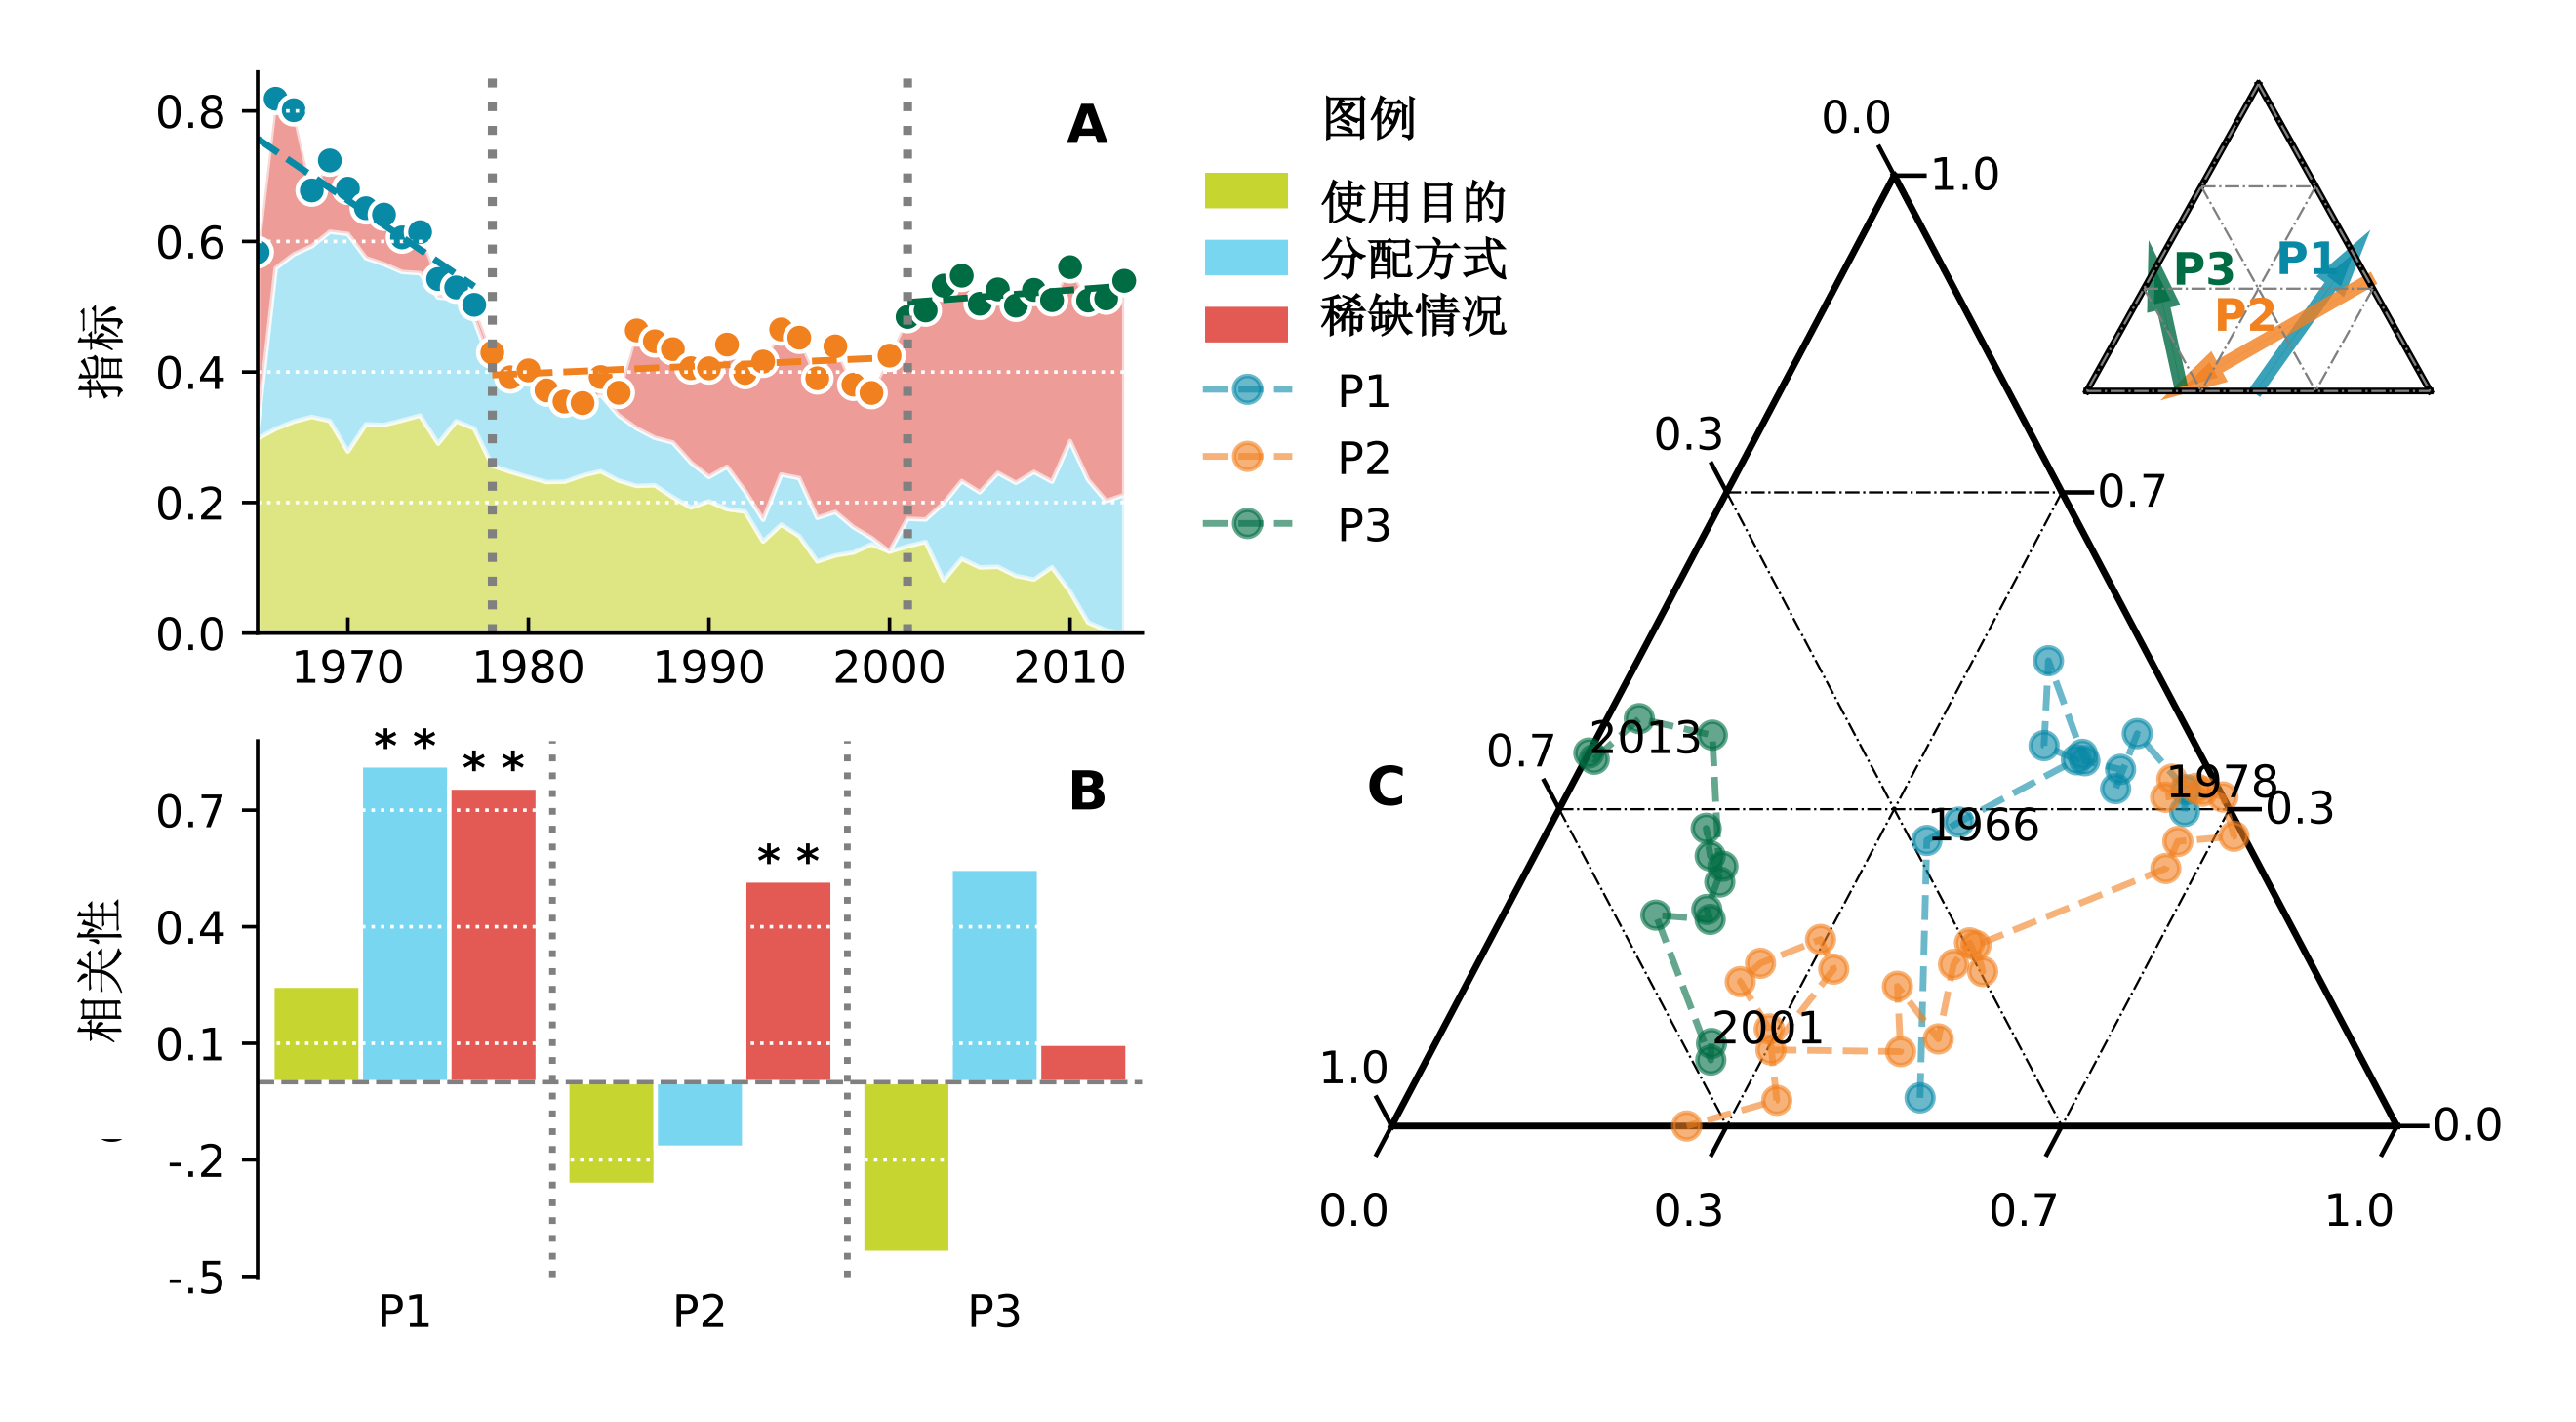
\includegraphics[width=\textwidth]{img/ch4/ch4_index.png}
	\caption[IWGI指数反映黄河流域的水治理变化阶段]{IWGI指数反映黄河流域的水治理变化阶段。两个突变点将1965年以来的黄河流域水治理划分为三个阶段,第一阶段(P1): $1965 \sim 1978$,第二阶段(P2): $1979 \sim 2001$,第三阶段(P3): $2002 \sim 2013$。
	\textbf{A,} 检测IWGI的突变点和三个指标的各自贡献:“稀缺情况(S)”、“使用目的(P)”和“分配方式(A)”。1978年和2001年出现了两个显著的变化点($p<0.01$)。
	\textbf{B,}  各阶段的IWGI变化与三个指标各自变化的相关性。
	\textbf{C,} IWGI随时间变化的同时,三个指标贡献比例的组合不断改变,致使水治理向不同方向发生阶段性转移。
	}\label{ch4:fig:IWGI}
\end{figure*}

IWGI在研究时段内存在两个突变点,将1965年以来的黄河流域水治理划分为三个阶段,第一阶段(P1): $1965 \sim 1978$,第二阶段(P2): $1979 \sim 2001$,第三阶段(P3): $2002 \sim 2013$,而“稀缺情况(S)”、“使用目的(P)”和“分配方式(A)”的三个指标在每个阶段的贡献不同(图~\ref{ch4:fig:IWGI}A)。
% 第一阶段
在第一个时期(P1, $1965 \sim 1978$)水资源压力对IWGI的贡献很小,“使用目的”和“分配方式”的指标的贡献更大(平均分别为$49.45\%$和$34.95\%$),但均呈现出显著的下降趋势($p<0.01$,图~\ref{ch4:fig:IWGI}~B),导致此时期IWGI迅速下降。
% 第二阶段
在第二阶段(P2, $1979 \sim 2001$),水资源压力指标的显著增加($p<0.01$)并为IWGI的略微上升做出主要贡献($p<0.01$,图~\ref{ch4:fig:IWGI}~A),而“使用目的”和“分配方式”的指标对IWGI的变化起了消极作用。
% 第三阶段
最后,在第三个时期(P3, $1995 \sim 2013$),尽管水资源压力指标在贡献中保持着$57.11\%$的最突出份额,但其数值已几乎保持不变,反而是“使用目的”的指标的降低和“分配方式”指标的增加,共同推动了综合指标IWGI的变化。
%的整体
综上所述,“稀缺情况(S)”、“使用目的(P)”和“分配方式(A)”的三个指标在不同时期对黄河流域水治理整体特征变化的贡献不同,将其演变历史划分为明显的三个阶段,依据其各自特点可命名为:集中供水时期、治理转变时期、适应增强时期(对应时间阶段分别为$1965 \sim 1978$、$1979 \sim 2001$、$2002 \sim 2013$(图~\ref{ch4:fig:IWGI}~C)。

\subsection{稀缺情况指标变化}

构成稀缺情况的指标(SFV指数)在研究时段(包括三个不同时期)内呈现出先降低、然后迅速增加、最后再次略微降低的变化趋势(图~\ref{ch4:fig:scarcity}~A)。
% ,表明水资源压力先减少再迅速增加,后趋于稳定
源区、上游、中游、下游这四个不同的区域中(图~\ref{ch4:fig:scarcity}~B),源区对三个时段的SFV指标变化几乎没有贡献,下游也仅在治理转变时期和适应增强时期呈现微弱的负向贡献。
对稀缺情况影响最大的是黄河的上游和中游,上游在集中供水时期和治理转变时期都是SFV变化的最大贡献区域,中游则在适应增强时期做出最大贡献。

\begin{figure}[!ht]
  \centering
  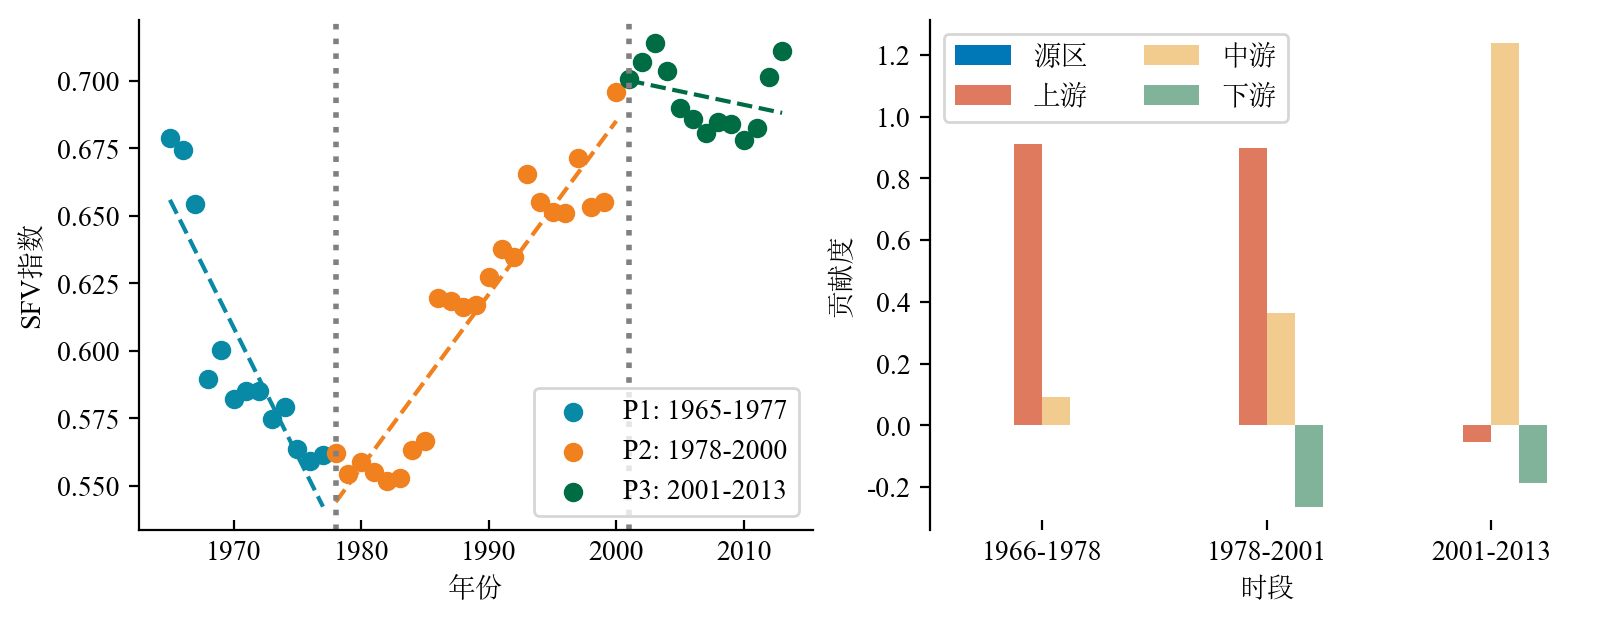
\includegraphics[width=\textwidth]{img/ch4/ch4_scarcity.png}
  \caption{稀缺性SFV指标变化趋势及各区域贡献}\label{ch4:fig:scarcity}
\end{figure}


\subsection{使用目的指标变化}

在用水目的上,供给性用水比例在集中供水时期基本保持不变,但在治理转变时期和适应增强时期呈现迅速下降的趋势(图\ref{ch4:fig:priority}~A)。
三个时段都是由灌溉用水的变化主导了该比例变化,城市、农村的人居用水、农村牲畜用水等几乎对该比例的变化没有影响(图\ref{ch4:fig:allocation}~B)。

\begin{figure}[!ht]
	\centering
	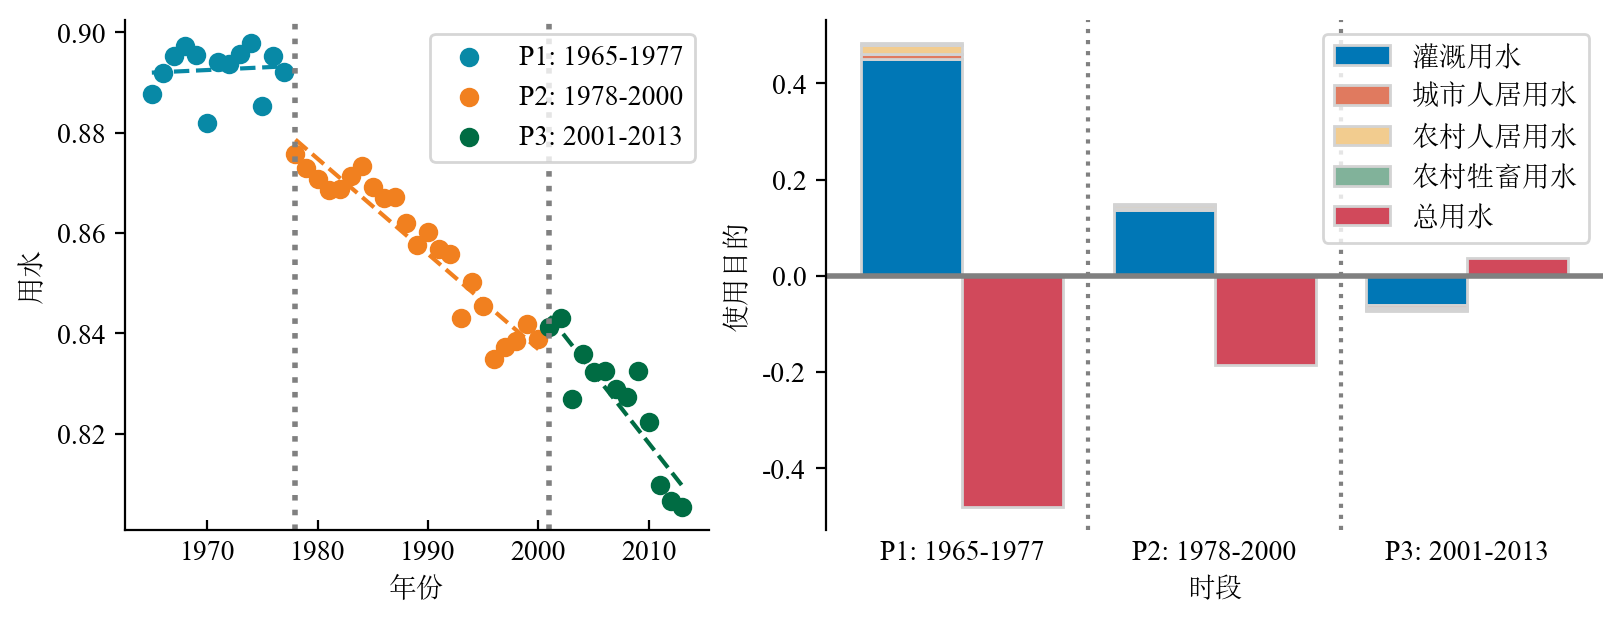
\includegraphics[width=\textwidth]{img/ch4/ch4_priority.png}
	\caption{供给性用水所占比例的变化趋势及各部门贡献}\label{ch4:fig:priority}
\end{figure}

\subsection{分配方式指标变化}

分配方式的指标变化呈现明显“V形”趋势,表明黄河的源区、上游、中游、下游之间水资源呈现先逐渐远离均匀分配,又在2000年后逐渐趋于平均的变化过程(图\ref{ch4:fig:allocation})。

\begin{figure}[!ht]
	\centering
	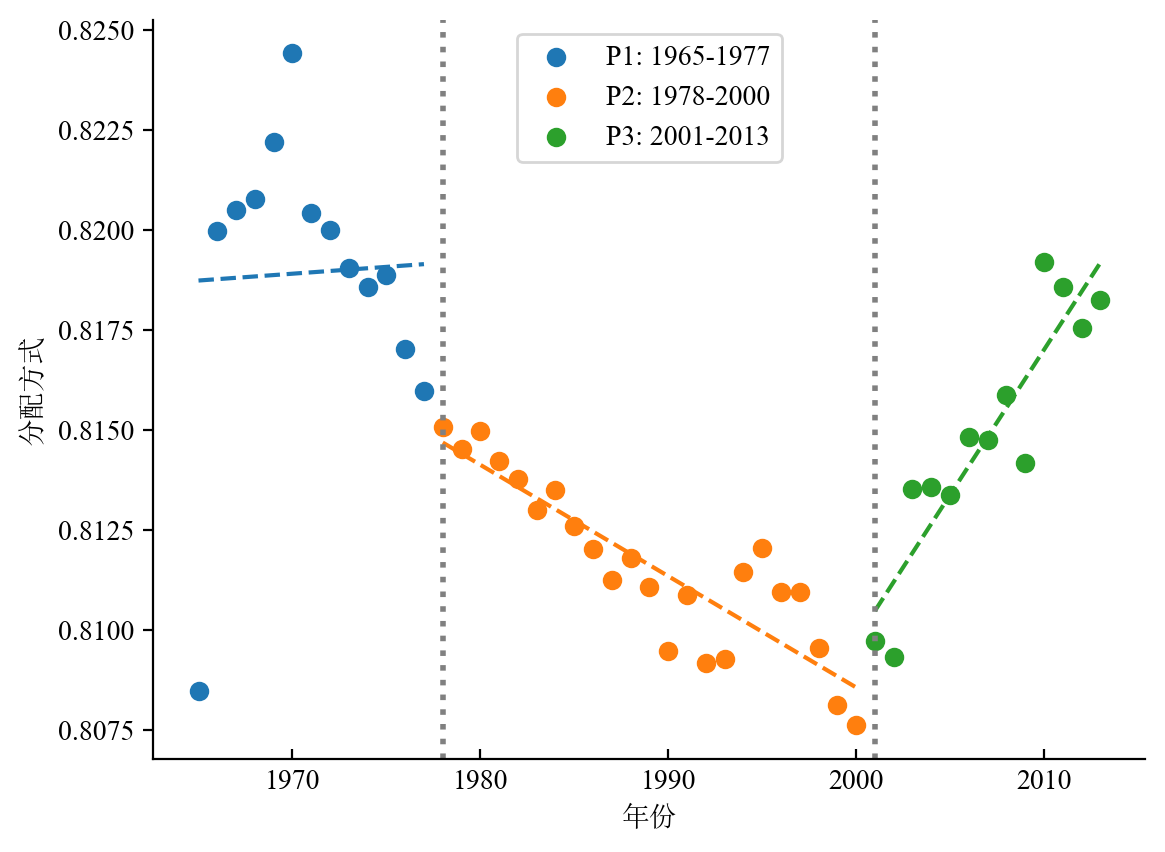
\includegraphics[width=0.6\textwidth]{img/ch4/ch4_allocation.png}
	\caption{分配方式指标的变化趋势}\label{ch4:fig:allocation}
\end{figure}

\section{人类活动主导时期人水关系演变机制}\label{ch4:mechanism}

% \subsection{水治理变化的驱动力分析}\label{ch4:sec:mechanism}

\begin{figure}[th!]
	\centering
	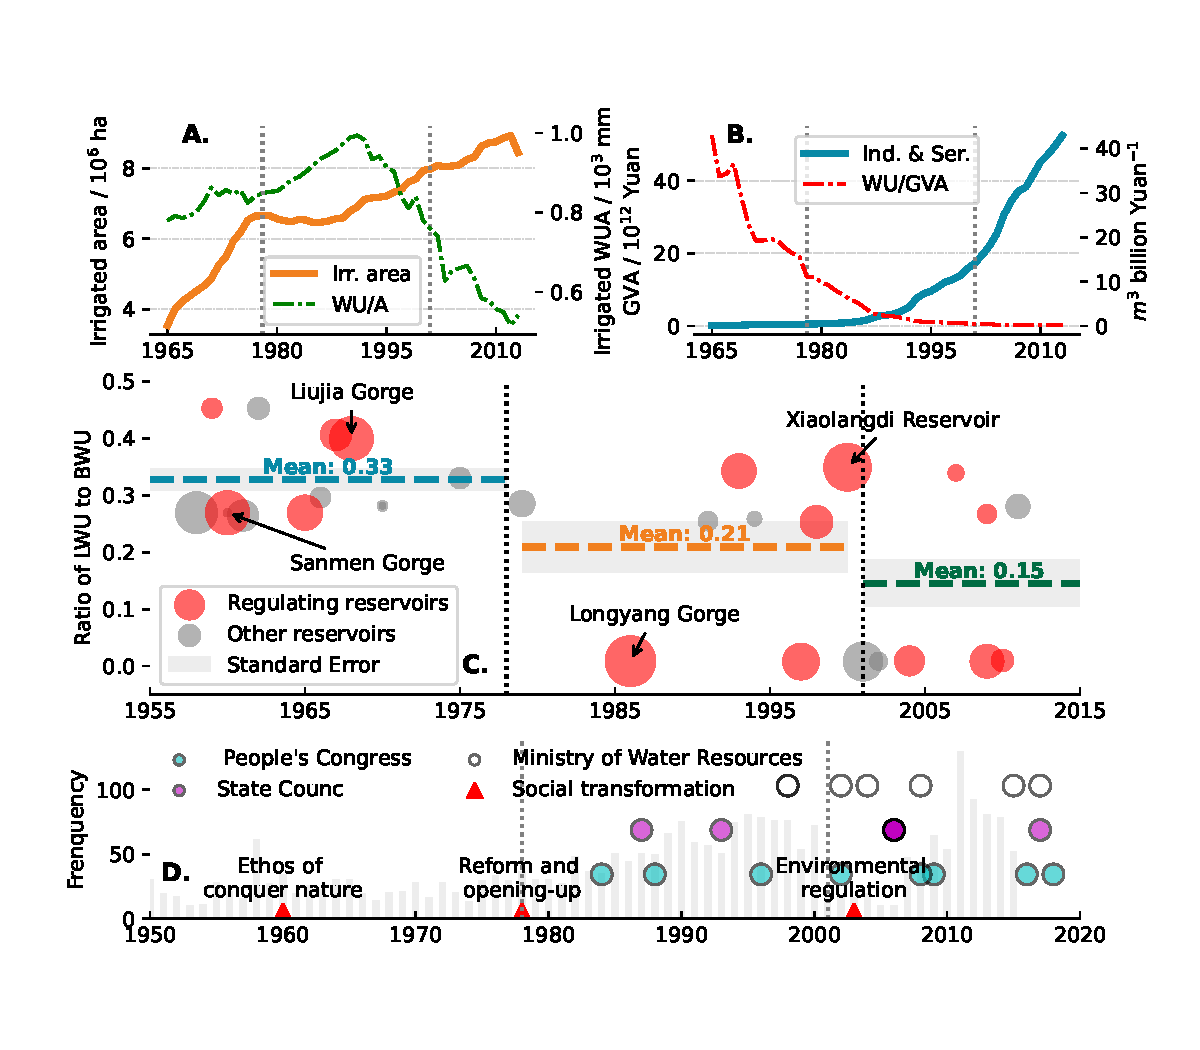
\includegraphics[width=\textwidth]{img/ch4/causes.pdf}
	\caption[黄河流域水治理阶段变化的驱动因素]{
		黄河流域水治理阶段变化的驱动因素。
		\textbf{A.}总灌溉面积($A$, 橙色线)和用水强度($WU/A$,用水量除以灌溉面积,绿点线)的变化。
        \textbf{B.}工业和服务业的总增加值(蓝线,$GVA$)变化及其用水强度($WU/GVA$,WU除以GVA,红点线)。
        \textbf{C.}每个水库的完工时间及其所在区域的用水量(Local Water Use, LWU)占水库完工时流域总用水量(Basinal Water Use, BWU)的百分比。红圈为负责黄河流域综合调度的水库。每个圆圈的大小表示其储水能力的大小。
        \textbf{D.}社会转型(红色三角形)和国家层面的治理政策(圆圈,不同颜色表示由不同的国家机构签署,越靠上代表国家机构的登记越高,详见表\ref{ch4:tab:policies})。浅灰色条形图以流域尺度(黄河大事件)计算与黄河流域有关的官方治理文献记录。}\label{ch4:fig:mechanism}
\end{figure}


\begin{figure}[tb]
    \centering
    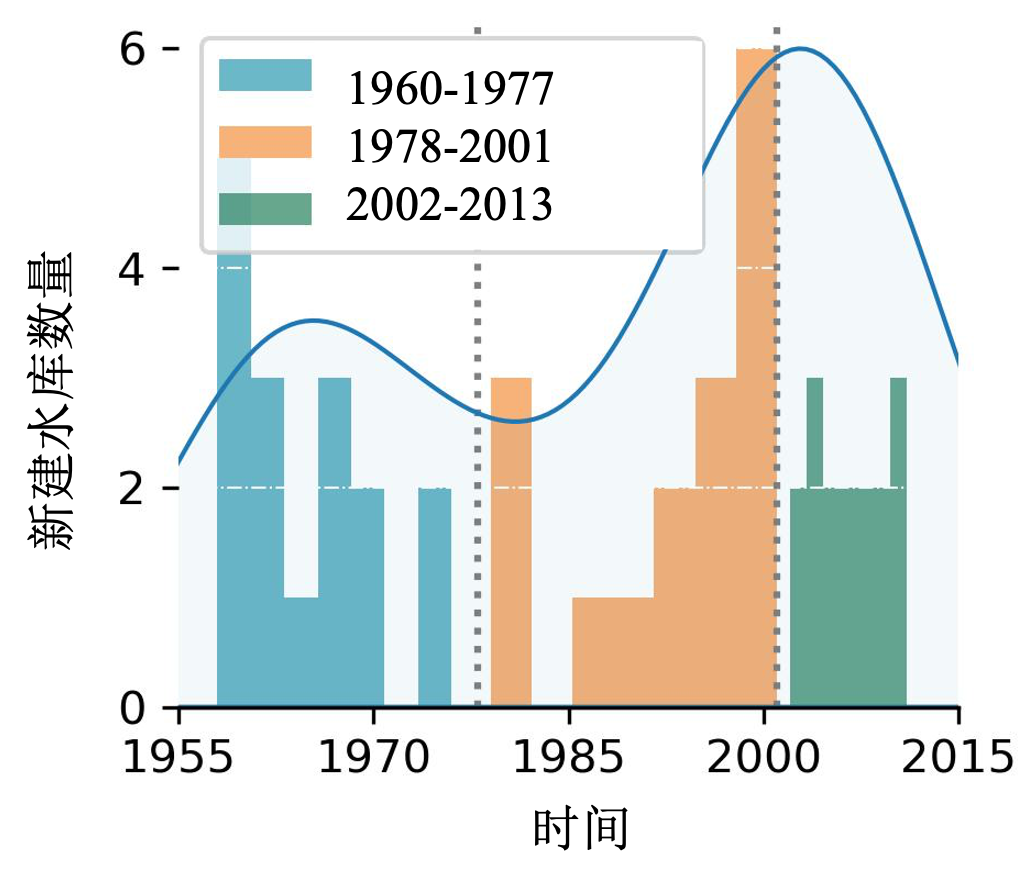
\includegraphics[width=0.6\linewidth]{img/ch4/ch4_reservoirs.png}
    \caption{黄河流域新增水库数量的时间分布}\label{ch4:fig:reservoirs}
\end{figure}


本节进一步探讨了致使IWGI变化的原因,灌溉区扩张和工业和服务业的经济增长是推动“集中供水时期”和“治理转变时期”两个阶段变化的关键。
黄河流域的用水需求在“集中供水时期”迅速增加,尤其是灌溉农业面积以$0.25*10^6 ha/yr$的速度迅速扩张(图\ref{ch4:fig:mechanism}~A),同时通过建设水库增加供应(图~\ref{ch4:fig:reservoirs})。
进入“治理转变时期”后,尽管灌溉区扩张停滞,但工业和服务业的发展开始增长,共同推动流域用水需求的进一步增加(图\ref{ch4:fig:mechanism}~A和B)。
接下来从“治理转变时期”到“适应增强时期”的演变过程中,水分利用效率变化最明显。
在“适应增强时期”,不仅工业和城市服务也承担了更重要的经济角色(由总增加值GVA表示,图\ref{ch4:fig:mechanism}~B),灌溉面积也恢复了缓慢扩张(图\ref{ch4:fig:mechanism}~A)。
但因用水效率的普遍提高,单位灌溉面积或单位产量的用水量都显著下降(图~\ref{ch4:fig:mechanism}~A和图~\ref{ch4:fig:mechanism}~B),因此部门和地区之间的用水差异在不断缩小,但流域水资源压力总体、持续维持在较高水平,公平合理分配宝贵水资源的压力越来越大(图~\ref{ch4:fig:IWGI}~A)。

最后,环境背景、社会文化、水治理政策等因素为三个时期的指标变化都产生了影响。
本研究首先计算了每个水库的区域用水量和流域用水量之比,较高的比值代表了该水库等潜在作用更有可能是旨在为该流域供水而不是流域调度;此外,流域调度的枢纽水库也以红色进行了标记(图~\ref{ch4:fig:mechanism}~C)。
可以看到,在阶段一的“集中供水时期”,受“人定胜天”的社会环境引领,大部分水库都建在需水量较大的地区,因此区域用水量和流域用水量之比值明显较高($p<0.01$,见图~\ref{ch4:fig:mechanism}~C)。
进入“治理转变时期”之后,新建水库的数量明显减少且多为枢纽水库,但全流域层次的法律法规(包括著名的“八七”分水方案)开始被不断提出,流域内的治理记录也迅速增加,可见此时期层出不穷的流域政策已深刻影响了流域水治理,流域水治理正在进行一场从工程措施向非工程措施的“治理转变”(图~\ref{ch4:fig:mechanism}~D, $p<0.01$和图\ref{ch4:fig:reservoirs})。
最后在“适应增强时期”,持续高位的水压力已成为制约区域发展的瓶颈,亟需通过节水转型和跨区域协调、调水来满足经济发展的用水需求,因此并且“大规模进行环境治理和节水转型”的国家战略指导下,有关部门提出了更多的、级别更高的水治理决策(图~\ref{ch4:fig:mechanism}~D)。
综上所述,从“集中供水时期”到“治理转变时期”的转变与当时水资源供需的增加相一致;而“治理转变时期”到“适应增强时期”的演变过程则是在水资源压力趋于稳定的同时,由社会监管政策和节水转型带来的效率提高所驱动的。

\section{讨论}\label{ch4:discussion}
\section{流域水治理演变模式}

研究结果显示黄河流域在人类主导时期有三种不同的流域治理模式:集中供水时期(P1: $1965 \sim 1978$)、治理转变时期(P2: $1979 \sim 2001$)和适应转向时期(P3: $2002 \sim 2013$)(图~\ref{ch4:fig:IWGI})。
在黄河流域水资源压力相对较低的集中供水时期($1965 \sim 1978$年),主要的水资源需求是为牲畜和作物等供给服务为目的,水治理也倾向于通过建造水库和引水渠等来增加水资源供给。
然而,正如当时“人定胜天”的口号所暗示的那样,水资源供应的增加并不能促进人-水关系和谐,因为它在不考虑生态保护的情况下急剧增加了用水,且这常常是一种不可逆转的变化\cite{zhou2020}。
在接下来的十年内,灌溉农田和引水设施的迅速扩张使黄河流域超负荷取水,在1972年以来,超过$80\%$的地表水被使用,导致河流频繁枯竭,造成了额外的生态问题,如湿地萎缩和生物多样性下降\cite{wang2019c}。
此外,由于水资源压力也限制了新兴的、更有利可图的工业与服务业的发展,这让流域的水治理模式接近了社会-生态危机的临界点,因为继续增加供应无论如何都是不切实际的\cite{loch2020, wohlfart2016a}。

治理体制转型时期的开始(P2: $1979 \sim 2001$)恰逢“改革开放”后,水资源竞争的持续加剧,但枯竭的黄河已经开始断流。
黄河流域在此时期开始水治理转变,这一结果与理论分析的结果高度一致:在流域总供应稳定的情况下,水资源需求在接近可供给水资源上限后的持续增长,将为流域水治理带来重大转型,流域社会-水文系统将通过制度措施让快速增强社会适应力,以响应该水资源供小于求的临界点\cite{loch2020}。
因此黄河流域在此时期发起了诸多水治理举措,包括控制灌溉面积的增长、倡导节水设施建设、制定全国首个水资源配额制度、并初步制定跨流域调水方案(南水北调)等\cite{wang2019b,long2020,nickum2021},成为了中国九大流域的制度变革先驱。
因此,尽管黄河流域的水资源压力仍然很大,且因径流减少和用水灵活性降低而持续增加,但黄河的断流问题却得到了解决,$1999$年的最后一次断流向世人昭示着此次水治理转变的巨大影响\cite{wang2019b}。

在随后的适应增强时期(P3: $2002 \sim 2013$)为适应稳定在高位的水资源压力,许多国家层面的黄河流域水治理实践都在这一时期提出,以期用最经济地方式,在保护生态的同时实现流域高质量发展。
二十一世纪初提出的“环境整治”和$2011$年提出的“最严格水资源管理”都是对水资源粗放式开发利用的响应,不断使流域水治理模式变得更高效。
这一时期除了中央政府主导的适应举措,地区各部门之间为了追求生产效率,社会经济过程为“水怎么用、水怎么分”的权衡发挥了重要作用。
典型的例子是黄河流域的水权转换工作,许多地区都积极推动了农业节水转型,并将节约的水额供给到经济效益更高的工业服务业之中。
通过不同行业和地区对流域水资源的广泛重建,通过日益强化的社会-经济过程调整以前粗放的发展模式以及刚性的制度约束,这些都是水治理适应性增强的体现,才能在有限的供水条件下优化平衡来自不同地区、不同行业的需求\cite{dalin2015,song2022}

黄河流域的水治理演化过程是“增大供给、治理转变、适应增强”的突出的案例,而其中变化的内在机制已在世界人类主导流域社会-水循环的过程中广泛出现(图~\ref{fig:summary})。
随着社会-经济过程对水循环影响加深,不同时期的流域面临不同的水治理挑战:在前期主要是经济和环境方面,在后期集中于与制度和政策方面。
放眼全球其它流域,以水资源短缺和供水困难为代表的水治理挑战是制约发展中流域的瓶颈\cite{allan2019,speed2013,liu2012a}。
人类社会-经济过程主导的发达流域(特别是跨界河流)则须重点解决结构性挑战,如水纠纷或缺乏公平\cite{mirumachi2015}。
本章研究开发并使用的综合水治理指数(IWGI)可以将流域水治理变化过程与这些挑战联系起来,提供了一种解释人类活动主导下人-水关系变化的方法。

\begin{figure}[htbp!]
	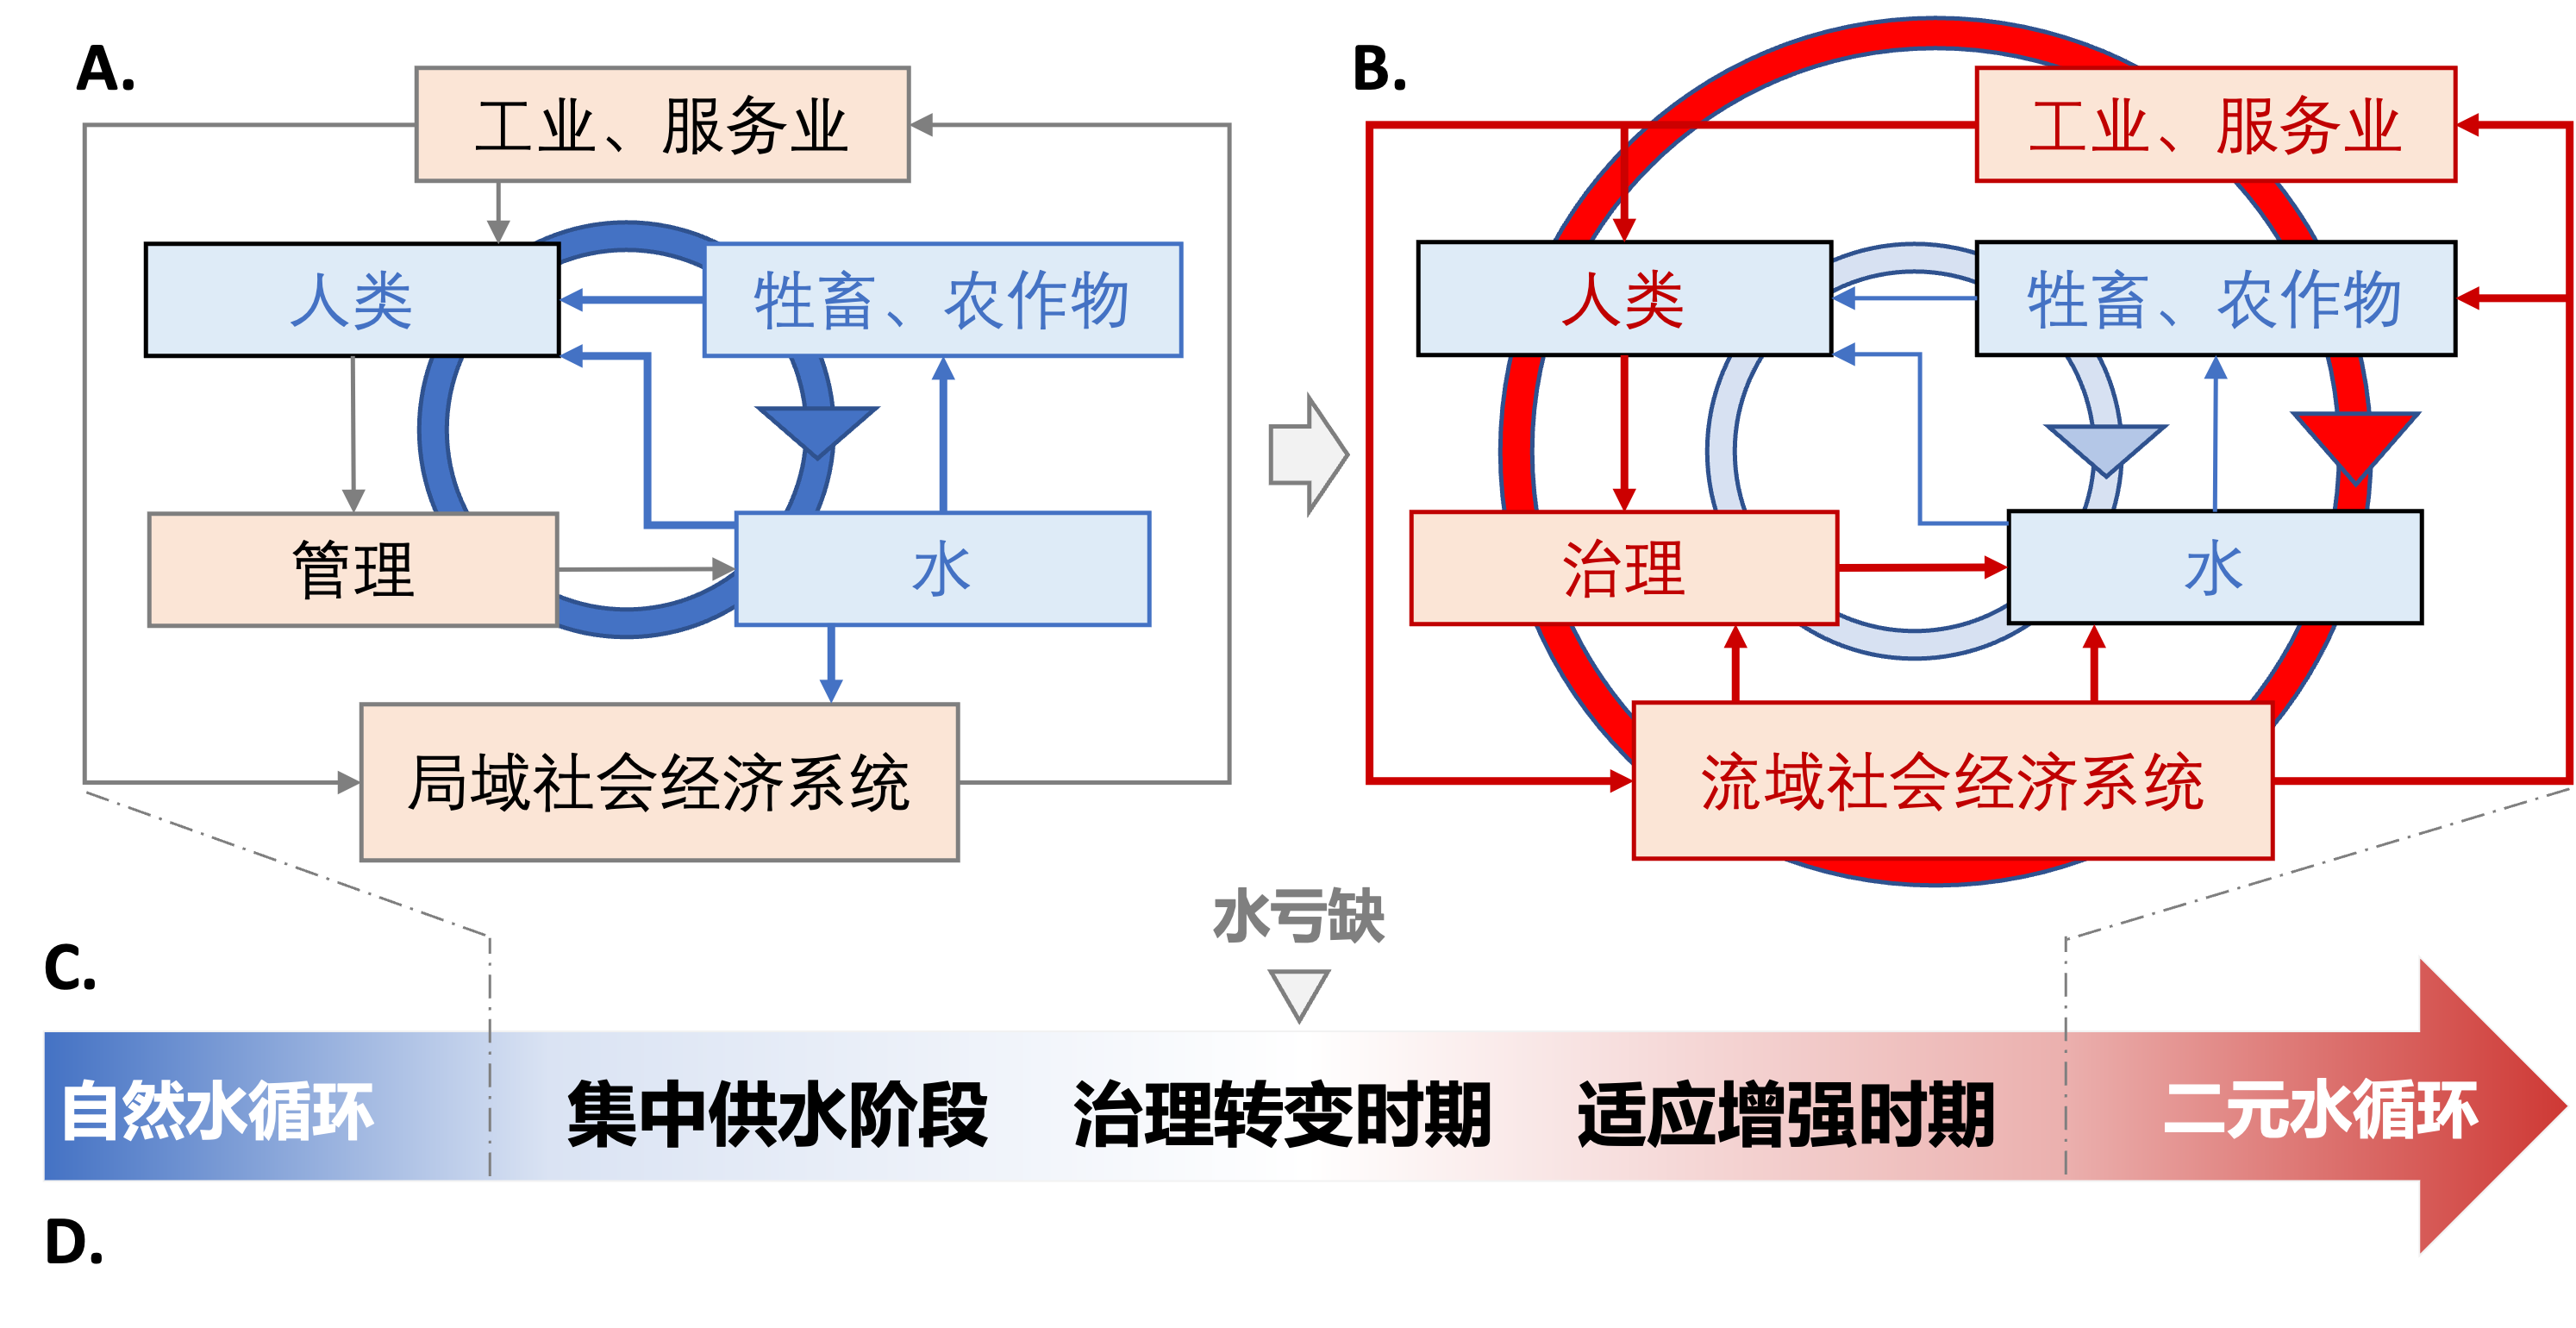
\includegraphics[width=\textwidth]{img/ch4/ch4_transition.png}
	\caption[人类主导下流域系统的水治理阶段过渡]{
		人类主导下流域系统的水治理变化过程。蓝色代表人类活动尚未成为主导的社会-水文循环,红色代表由社会经济过程主导的流域水过程。
        \textbf{A.}随着社会经济系统的发展,用以非供给服务的水需求增加;同时,通过水库等工程措施使人们能够控制水循环并局部缓解水资源压力。
        \textbf{B.}随着人为干预升级,不同地区和部门间的用水权衡愈发突出;流域亟需提升利用效率和调度能力,并组织起的更具适应性的水治理。
        \textbf{C.}在人类主导的流域社会-水文循环模式下,水治理转变常发生在水资源亏缺之后,在社会-经济过程主导下推动适应能力快速增长。在此之前水治理主要面临经济和环境挑战,但随后面临社会和政策挑战。
	}\label{fig:summary}
\end{figure}

\section{对流域治理规律的启示}

通过在数据丰富的黄河流域进行应用,本章研究表明所有的水治理问题都会导致“谁获得水、何时获得水以及如何获得水”的改变,因此监测“有多少水、怎么用、怎么分”三个关键问题对识别流域水治理变化有极大帮助。
但在世界范围内广泛应用该方法的主要局限是缺乏全球尺度的长时间序列数据,这意味着IWGI的可能缺点是难以推广。
在数据相对不足的流域应用IWGI时,建议不同方面的指标选择可根据现有数据集进行调整,因为底层指标之间关系的变化趋势比精确计算指标更重要。
在当今这个“人类世”,人-水关系由人类活动所主导的情况越来越普遍,应对层出不穷的治理挑战已成为复杂的人-水系统的核心\cite{cumming2018,cumming2014,jaeger2019}。
许多流域仍在不断接近系统随时可能崩溃的“地球界限”\cite{gleeson2020, wang-erlandsson2022},只有更深入地理解流域水治理系统,结合非线性稳态变化和转型的思想,才能维持流域社会-生态系统的韧性并实现可持续、高质量发展\cite{falkenmark2019}。

% Implications
由于大型河流流域是生态系统服务、经济发展和人类福祉的关键来源,水治理逐渐从主要的地方问题成为国家或国际问题\cite{best2019,best2020}。
随着远程耦合在联系日益紧密的世界中提出了更多的水治理挑战,水治理的政权转变与不同的人与水的关系相一致\cite{diaz2019}。
这一过程反映了社会如何通过增强其在水社会循环中的适应能力来改变治理实践的建议,IWGI定量地确定了这一转变\cite{loch2020,turton1999}。
科学家和决策者认识到不断变化的治理挑战是至关重要的,因为在一个阶段下开发的模型、制度、工程和方法不一定适用于另一个治理阶段\cite{reyers2018}。


\section{小结}\label{ch4:summary}
% 本章整合了水文数据、统计数据、历史文献材料等多源数据,开发流域水治理综合指数(Integrated Water Governance Index, IWGI),利用突变点检测方法量化识别了二十世纪六十年代以来的黄河流域治理的阶段变化,并分析了转变发生的驱动因素。

本章研究表明,两个突变点可以将1965 - 2013 年的黄河流域水治理演变历史划分为明显的三个阶段,依据其各自特点可命名为:集中供水时期(1965 - 1978,P1)、治理转变时期(1979 - 2001,P2)、适应增强时期(2002 - 2013,P3),而“稀缺情况(S)”、“使用目的(P)”和“分配方式(A)”的三个方面的指标在各阶段为黄河流域水治理的特征变化做出了不同贡献。
进一步探讨致使IWGI变化的原因,灌溉区扩张及工业和服务业的经济增长是推动“集中供水时期”和“治理转变时期”两个阶段变化的主要原因,环境背景、社会文化等因素对不同阶段的指标变化都产生了影响,水治理政策是将“治理转变时期”推向“适应增强时期”的主要驱动力。

黄河流域的水治理演化过程是“增大供给、治理转变、适应增强”的突出的案例,而其变化规律已在全球由人类主导的流域社会-水文循环过程中广泛出现。
理解黄河流域水治理的变化规律,可以为快速变化的大河流域提供实现可持续性的重要理论依据。

% Implications
由于大型河流流域是生态系统服务、经济发展和人类福祉的关键来源,水治理逐渐从主要的地方问题成为国家或国际问题\cite{best2019,best2020}。
随着远程耦合在联系日益紧密的世界中提出了更多的水治理挑战,水治理的政权转变与不同的人与水的关系相一致\cite{diaz2019}。
这一过程反映了社会如何通过增强其在水社会循环中的适应能力来改变治理实践的建议,IWGI定量地确定了这一转变\cite{loch2020,turton1999}。
科学家和决策者认识到不断变化的治理挑战是至关重要的,因为在一个阶段下开发的模型、制度、工程和方法不一定适用于另一个治理阶段\cite{reyers2018}。
